\chapter{Planteamiento del Problema}
\section{Descripción de la Realidad Problemática}

En la actualidad, cada vez es más necesario el uso de la conectividad a internet como método de interacción entre los usuarios, empresas e instituciones educativas, convirtiéndose en un instrumento imprescindible para las actividades relacionadas a ella. En la mayoría de las empresas no se cuenta con una cobertura de la red Wi-Fi total que garantice el acceso a internet y es allí donde surgen muchos inconvenientes tanto para el envío de trabajos, realización de consultas, entre otras actividades en las que la red sería de gran ayuda.

Lograr encontrar la ubicación idónea de Aps Indoor para lograr la cobertura total de un lugar es un proceso iterativo que consume mucho tiempo, que requiere múltiples rondas de refinamientos. Un especialista de TI esboza un diseño, evalúa, ajusta y repite los ciclos hasta estar satisfecho con un diseño dentro de un presupuesto de tiempo dado. Desafortunadamente, diseñar un plano de cobertura de red efectivo solo es posible mediante especialistas de TI o Redes, donde gran parte de empresas hacen su propio diseño personalizado menos efectivo debido al costo. La generación automática de planos de cobertura de red con las ubicaciones de Aps Indoor tendrá un tremendo impacto en las industrias de bienes raíces/construcción, redes y TI de billones de dólares.

En los últimos años, ha habido un aumento en la demanda de redes inalámbricas entre los usuarios, gracias a los beneficios que ofrecen en términos de movilidad y costos de implementación más bajos. Dentro de las redes inalámbricas, se encuentran las WLAN (Redes de Área Local Inalámbricas), las cuales son comúnmente utilizadas en entornos cotidianos como hogares, oficinas y instituciones educativas, entre otros lugares. Estas redes suelen estar compuestas principalmente por dispositivos concentradores conocidos como Puntos de Acceso (AP), los cuales permiten a los usuarios conectarse de forma inalámbrica a la red, cumpliendo una función similar a la de un Switch en una red cableada. Sin embargo, a pesar de la capacidad de los AP para establecer conexiones inalámbricas, la distancia efectiva entre el usuario y el AP es limitada (generalmente inferior a 100 metros), debido a la potencia de la señal de transmisión y a posibles obstáculos en el entorno que puedan afectar la señal. Debido a la creciente necesidad de conectividad inalámbrica por parte de los usuarios, la cantidad de Puntos de Acceso en uso está en constante aumento.

Según una investigación realizada por ABI Research, compañía que asesora a fabricantes del mundo de los semiconductores sin cable, en 2026 se llegará al despliegue total de Wi-Fi 6, el cual se acelera rápidamente mucho más allá de los dispositivos Wi-Fi insignia, cada vez más dispositivos admiten la banda de 6 GHz está integrado en un número cada vez mayor de dispositivos de consumo convencionales. (Zignani et al., 2022) Ello es algo que se debe tener, en cuenta debido al rápido avance de la tecnología y a las consecuencias que estas tendrán.

En un artículo del diario El País, se destaca un problema creciente relacionado con la conectividad Wi-Fi en los hogares. A medida que más dispositivos se conectan a las redes inalámbricas, la infraestructura existente se ve sometida a una presión cada vez mayor. Además, muchos hogares y empresas aún utilizan enrutadores y puntos de acceso antiguos que no pueden manejar la cantidad de dispositivos conectados, sumando la falta de actualización de la infraestructura contribuye al problema.(El País, 2023)

Según el Instituto Nacional de Estadística e Informática (INEI), en el primer trimestre de 2022, el 95,0\% de los hogares del país tenían al menos un servicio de Tecnología de Información y Comunicación (TIC). Este indicador muestra un crecimiento de 0,2 y 1,9 puntos porcentuales, al compararlo con el mismo trimestre de los años 2021 y 2019, respectivamente. (INEI, 2022)

En el ámbito de las redes inalámbricas, especialmente en entornos corporativos y de alta demanda, como los clientes de Cisco, las quejas sobre la conectividad y el rendimiento de las WLAN (Wireless Local Area Network) son una constante preocupación. A medida que aumenta la dependencia de estas redes para la comunicación, colaboración y operaciones empresariales, también lo hacen los desafíos técnicos y las expectativas de los usuarios. Uno de los problemas recurrentes es la cobertura inalámbrica insuficiente, que se manifiesta en áreas muertas donde la señal es débil o inexistente. Esto puede deberse a la ubicación subóptima de los puntos de acceso (AP) o a interferencias externas que obstaculizan la propagación de la señal. Los clientes de Cisco a menudo expresan su frustración por tener que moverse dentro de un espacio para obtener una señal sólida, lo que afecta negativamente la productividad y la experiencia del usuario. (Foro de Cisco, 2023)

\begin{figure}[h]
	\begin{center}
		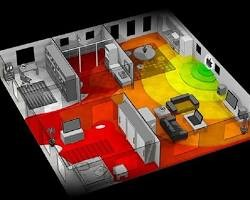
\includegraphics[width=0.55\textwidth]{1/figures/CISCO_QUEJAS.jpg}
		\caption[Quejas de Clientes en el foro de Cisco]{Quejas de Clientes en el foro de Cisco\\
		Fuente: \cite{cr_hustle2019successrate}. \textit{Cobertura de red ineficiente}}
		\label{1:fig2}
	\end{center}
\end{figure}

Además de este problema, en muchos casos los usuarios optan por adquirir un nuevo punto de acceso para mejorar el medio ambiente, pero esto puede tener consecuencias negativas. La compatibilidad entre los dispositivos instalados no siempre está garantizada y también puede haber incompatibilidades a nivel de switch y VPN. Identificar y resolver estos problemas de una manera que tenga o tenga menos impacto en las operaciones requiere un sólido conocimiento técnico en el campo de las tecnologías de la información (TI), ya sea dentro del negocio o mediante el uso de servicios tecnológicos especializados. El procesamiento lento genera, entre otras desventajas, la necesidad de retrabajo, demoras en la emisión de informes y documentos y costos adicionales relacionados con las horas extras. (Napit, 2017)

A lo anterior, podemos sumar que los errores de configuración en switches, enrutadores y puntos de acceso también pueden tener un impacto negativo en la red inalámbrica, provocando, por ejemplo, ralentizaciones y caídas de conexiones. Por lo tanto, reconfigurar estos dispositivos puede ayudar a abordar los desafíos de la red. Una solución eficaz a esta situación es realizar un análisis detallado del entorno y las estructuras existentes. Con esta evaluación, resulta más fácil determinar la ubicación adecuada para conectar los elementos, evaluar los requisitos de los nuevos componentes y garantizar que sigan funcionando de manera óptima. (Napit, 2017)

\begin{figure}[h]
	\begin{center}
		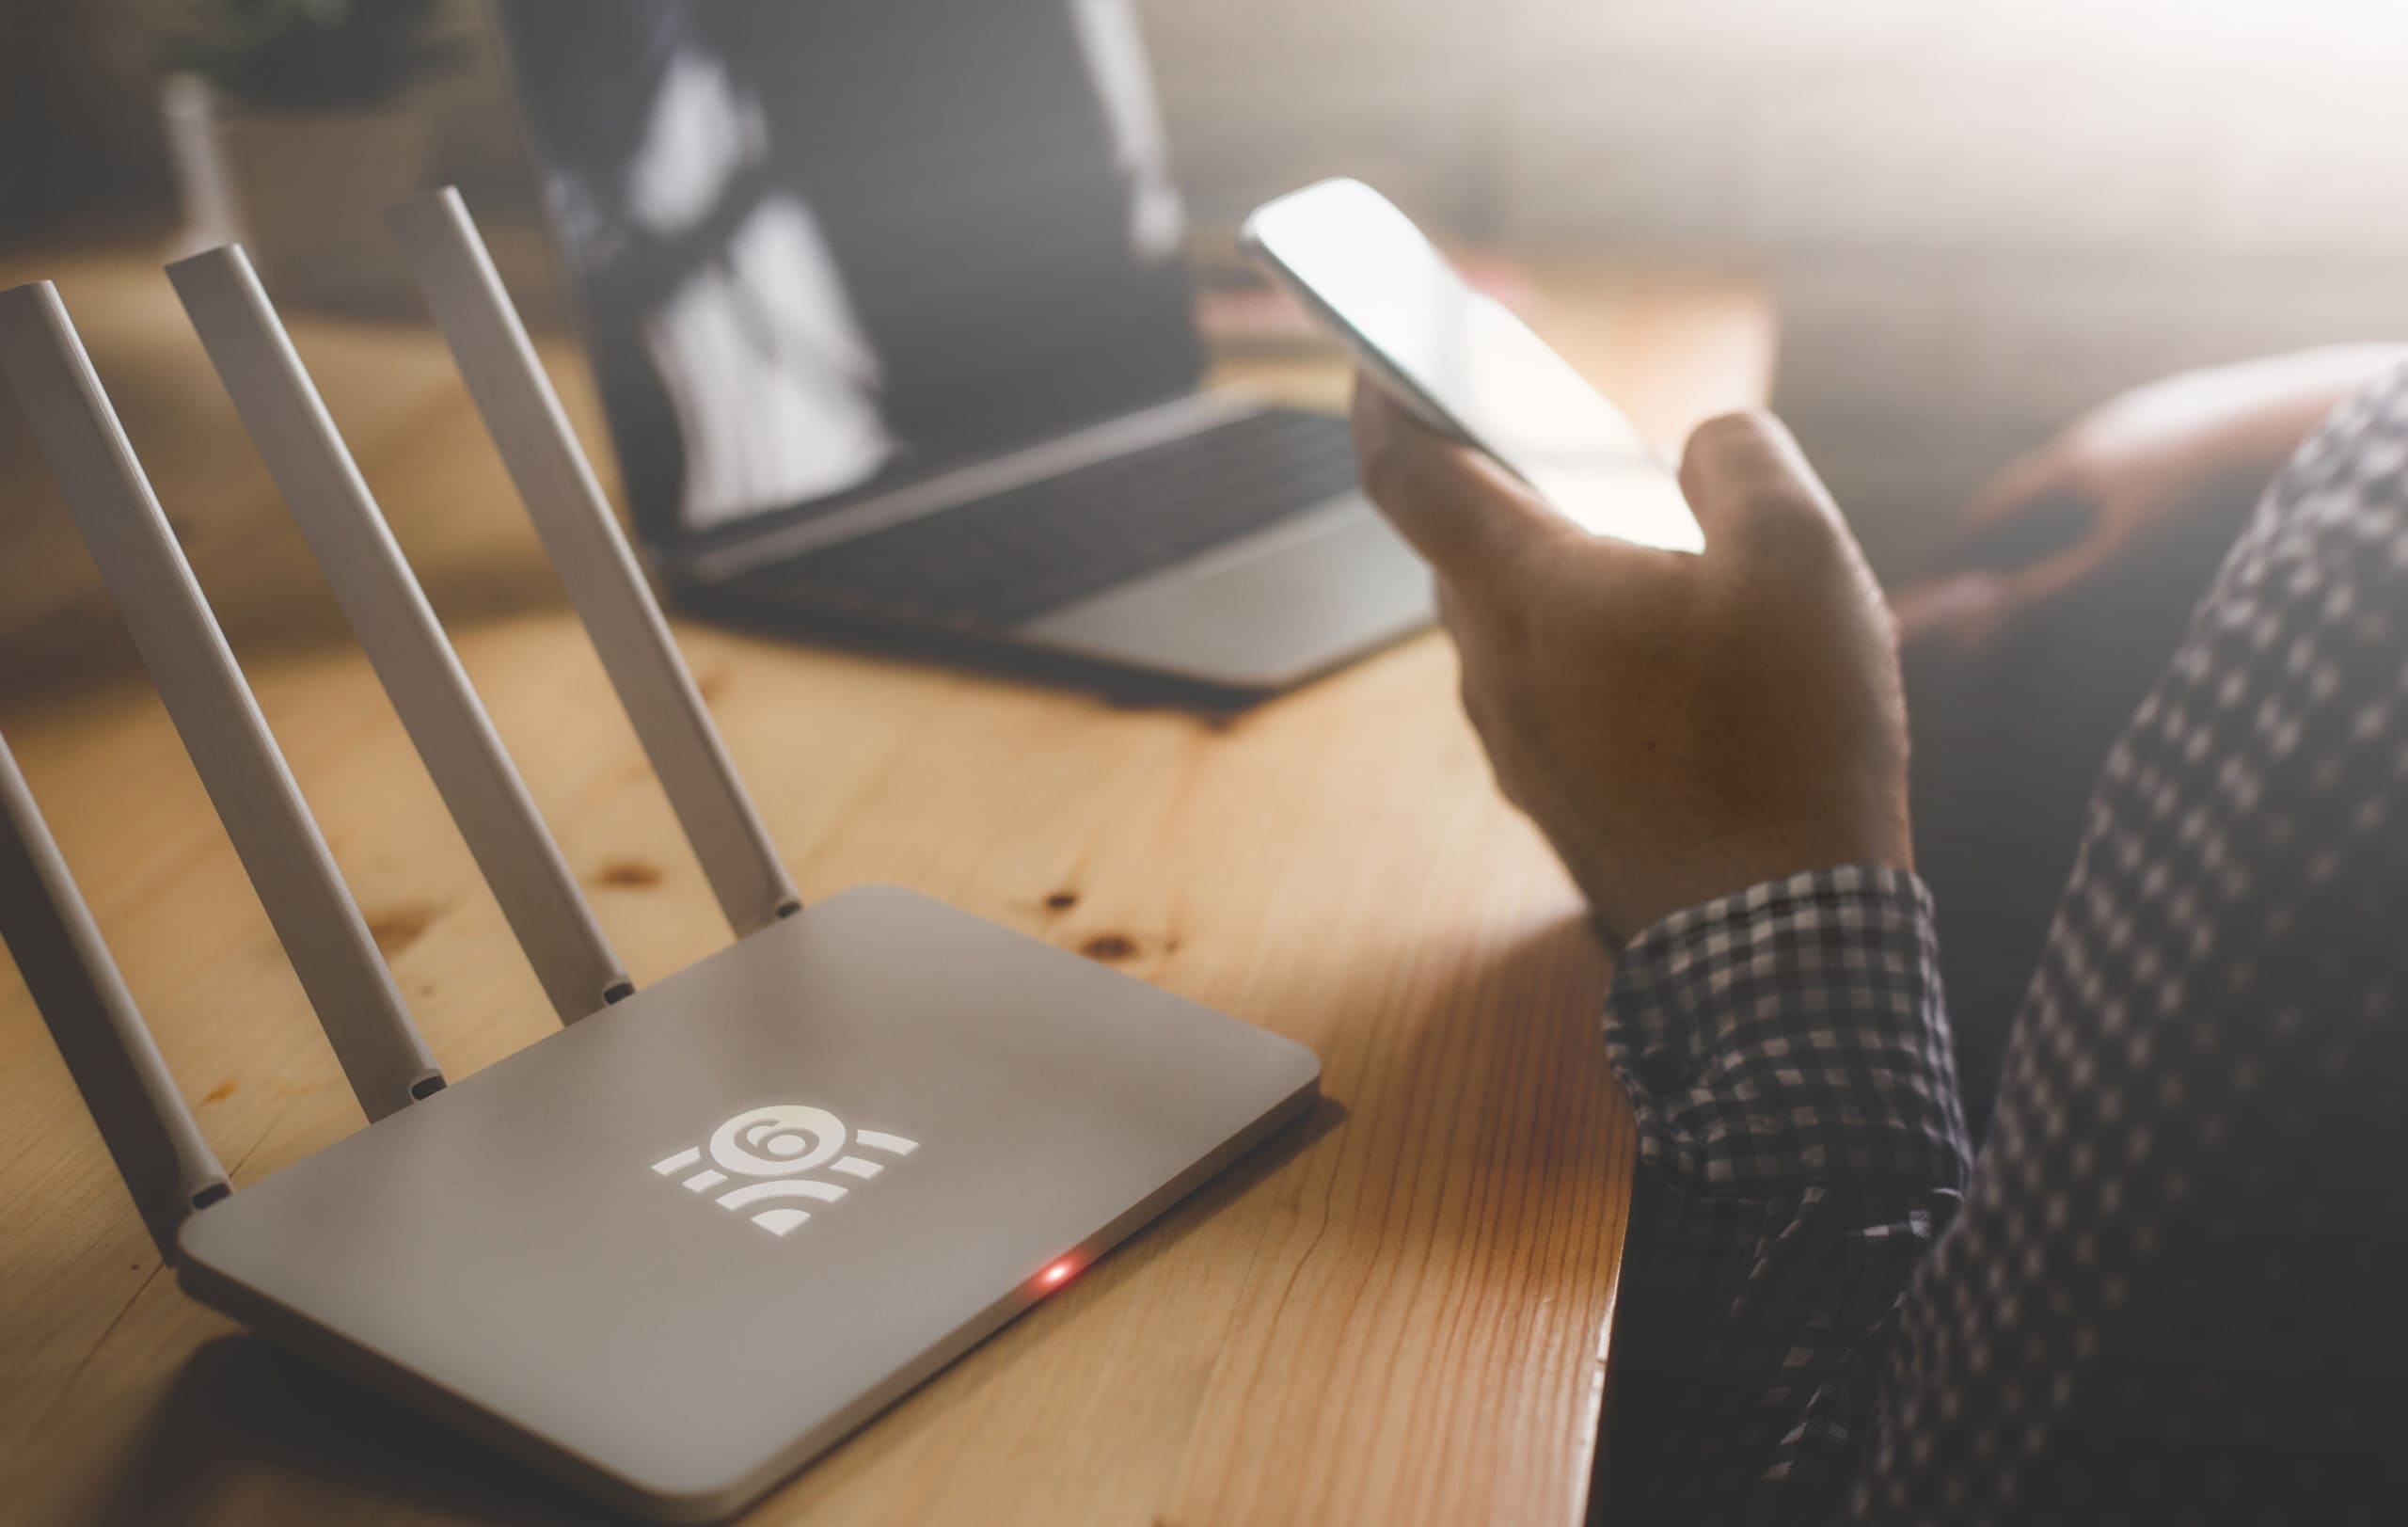
\includegraphics[width=0.55\textwidth]{1/figures/access-point-1.jpeg}
		\caption[Problemas de uso de Access Points]{Problemas de uso de Access Points\\
		Fuente: \cite{cr_hustle2019successrate}. \textit{Problema con el funcionamiento ideal del Access Point}}
		\label{1:fig2}
	\end{center}
\end{figure}

\section{Formulación del Problema}
Para la formulación de los problemas de la presente investigación, se elaboró un «árbol de problemas» (véase Anexo \ref{anexo1}).

\subsection{Problema General}
PG: \newcommand{\ProblemaGeneral}{
¿Es posible predecir las ubicaciones de Puntos de Acceso (APs) Indoor en Diferentes Planos  mediante Inteligencia Artificial Generativa?
}
\ProblemaGeneral
\subsection{Problemas Específicos}
\newcommand{\Pbone}{
¿Cómo se puede modelar de manera efectiva la distribución espacial de usuarios y obstáculos en un entorno interior para predecir la cobertura inalámbrica?
}
\newcommand{\Pbtwo}{
¿Qué enfoques de inteligencia artificial generativa, como redes generativas adversarias (GANs) o modelos de generación de texto, son más adecuados para generar ubicaciones óptimas de APs en entornos interiores?
}
\newcommand{\Pbthree}{
¿Qué estrategias de optimización se pueden aplicar para ajustar dinámicamente los recursos, como la potencia de transmisión y la capacidad de los APs, con el fin de mejorar la calidad de la cobertura inalámbrica?
}
\newcommand{\Pbfour}{
¿Cómo se pueden equilibrar eficientemente los recursos asignados a diferentes APs para garantizar una cobertura uniforme y una distribución equitativa de la capacidad de red?
}

\begin{itemize}
	\item PE1: {\Pbone}
	\item PE2: {\Pbtwo}
	\item PE3: {\Pbthree}
	\item PE4: {\Pbfour}
\end{itemize}

\section{Objetivos de la Investigación}
Para la formulación de los objetivos de la presente investigación, se elaboró un «árbol de objetivos» (véase Anexo \ref{anexo2}) 
\subsection{Objetivo General}
OG: \newcommand{\ObjetivoGeneral}{
Desarrollar y aplicar técnicas de inteligencia artificial generativa para predecir las ubicaciones óptimas de puntos de acceso (APs) en diferentes planos de un entorno interior, con el fin de optimizar la cobertura de redes inalámbricas y mejorar la conectividad y calidad del servicio para los usuarios finales.
}
\ObjetivoGeneral
\subsection{Objetivos Específicos}
\newcommand{\Objone}{
Desarrollar un algoritmo que pueda simular con precisión la cobertura de redes inalámbricas en interiores
}
\newcommand{\Objtwo}{
Implementar un modelo generativo capaz de proponer automáticamente ubicaciones eficientes para los Aps
}
\newcommand{\Objthree}{
Desarrollar algoritmos de optimización que ajusten dinámicamente los parámetros de los APs para mejorar la eficiencia del sistema.
}
\newcommand{\Objfour}{
Desarrollar e implementar un algoritmo de balanceo de carga dinámico para optimizar la asignación de recursos entre los diferentes puntos de acceso (APs) de una red inalámbrica.
}

\begin{itemize}
	\item OE1: {\Objone}
	\item OE2: {\Objtwo}
	\item OE3: {\Objthree}
	\item OE4: {\Objfour}
\end{itemize}

\section{Hipótesis}

\subsection{Hipótesis General}
HG: \newcommand{\HipotesisGeneral}{
	El modelo de Aprendizaje Profundo Multimodal predecirá el estado de financiamiento de proyectos de tecnología en sitio web de crowdfunding Kickstarter.
}
\HipotesisGeneral
\subsection{Hipótesis Específicas}
\newcommand{\Hone}{
El análisis de las alternativas propuestas en los trabajos previos influirá en la selección de características y desarrollo del marco de trabajo de la investigación.
}
\newcommand{\Htwo}{
La factibilidad técnica del ambiente de desarrollo para las características del modelo de Aprendizaje Profundo Multimodal determinará la aplicabilidad de las condiciones de las propuestas de la literatura.
}
\newcommand{\Hthree}{
El modelo de Aprendizaje Profundo Multimodal se verá afectado por las características consideradas en su desarrollo.
}
\newcommand{\Hfour}{
La herramienta analítica implementada ayudará en tiempo real a los emprendedores y creadores de proyectos de tecnología en la toma de decisiones y estrategias de sus campañas.
}

\begin{itemize}
	\item HE1: \Hone
	\item HE2: \Htwo
	\item HE3: \Hthree
	\item HE4: \Hfour
\end{itemize}

Los problemas, objetivos e hipótesis descritas anteriormente se encuentran alineados en la Matriz de Consistencia del Anexo \ref{anexo3}. Además, los objetivos específicos se formularon a partir de una lluvia de ideas luego de examinar los objetivos planteados en los antecedentes, cuyo detalle e item de referencia se encuentra en el Anexo \ref{anexo5}.

\section{Justificación de la Investigación}

\subsection{Teórica}
Esta investigación se realizó con la finalidad de aportar al conocimiento existente del problema de la predicción del estado de financiamiento de un proyecto en plataformas de crowdfunding como Kickstarter, pero considerando solo proyectos de la categoría Tecnología, cuyo ratio de éxito de 20\% la clasifica como la más baja de todas, criterio que también se menciona en la literatura por \cite{pr_lee2018contentDL}.

Para ello, el nuevo aporte aplicado a la investigación fue la implementación de un modelo de Aprendizaje Profundo Multimodal utilizando la información de la sección principal de la campaña (metainformación y descripción) y los comentarios de los patrocinadores como resultado de la interacción entre ellos y los creadores. Esta nueva perspectiva considera las 3 modalidades más utilizadas en los antecedentes bajo un modelo que solo fue desarrollado en 1 antecedente por \cite{pr_cheng2019deeplearning}, el cual utilizó solo modalidades de la sección principal (metainformación, descripción e imagen del proyecto).

\subsection{Práctica}
Muchos trabajos previos analizados en la literatura plantearon distintas soluciones para resolver el mismo problema. Sin embargo, a pesar de que sus resultados en su mayoría alcanzaron niveles de predicción por encima a los esperados por los autores, menos de la mitad (8 de los 18 antecedentes mencionados) llegaron a ejecutar la fase de Despliegue, es decir, no fueron puestos en producción para ser utilizados por otros usuarios, o se mencionaron que se convertiría en una tarea para trabajos a futuro.

Al culminar esta invesigación, se podrá utilizar el prototipo de un sistema que integra el modelo propuesto, el cual funciona en tiempo real capturando la información de las variables solamente recibiendo como entrada la URL del proyecto, con la finalidad de poder ser una herramienta analítica de ayuda en la toma de decisiones a emprendedores que buscan financiar sus proyectos de tecnología en Kickstarter. La retroalimentación será recíproca entre el usuario y el prototipo, ya que en la primera iteración, el creador tendrá una idea inicial del resultado de éxito de financiamiento que tendrá su campaña de acuerdo a la información actual presente en sus variables, y ante una respuesta adversa, podrá realizar las modificaciones respectivas en las modalidades entrenadas que tiene acceso (metainformación y descripción) para ejecutar nuevamente el prototipo, que ahora hará la predicción a partir de nuevos datos, de forma indefinida. De esta manera, se logrará crear una campaña más atractiva para los patrocinadores.

\subsection{Metodológica}
La implementación del modelo propuesto ayudará a los emprendedores y creadores a evaluar las campañas de sus proyectos a partir de la información vigente que sea capturada en tiempo real por el prototipo para predecir el estado de financiamiento.

Para ello, se utilizaron técnicas de Aprendizaje Profundo y Procesamiento de Lenguaje Natural entrenados con un conjunto de datos compuesto por 3 modalidades de proyectos en Kickstarter que fueron generados luego de un proceso de recolección de datos.

\section{Delimitación del Estudio}

\subsection{Espacial}
Para la presente investigación, se consideraron proyectos de tecnología de distintas ciudades y países, mayoritariamente del territorio de los Estados Unidos. Sin embargo, la información textual (descripción y comentarios) para la fase de entrenamiento solo se tómo en cuenta palabras en inglés.

\subsection{Temporal}
El periodo de tiempo abarcará desde el año 2009, fecha en el cual se tiene registrado los primeros conjuntos de datos de proyectos en Kickstarter hasta el mes de agosto del año 2019, últimos registros descargados hasta el inicio del presente trabajo.

\subsection{Conceptual}
Esta investigación se orientará en la implementación de un modelo que logre predecir si un proyecto de tecnología en el sitio web de crowdfunding Kickstarter será financiado o no. Para ello, se valió del uso de herramientas de Aprendizaje Profundo y Procesamiento de Lenguaje Natural para desarrollar los modelos de acuerdo a sus modalidades respectivas, así como el Aprendizaje Profundo Multimodal para consolidar estos conceptos.